%\documentclass[handout]{beamer}
\documentclass[presentation]{beamer}
\setbeameroption{show notes}

% Options for the UBD theme
\usetheme[
%	progressdots,  % provides progress dots by sections at the top of each slide
	transitions,  % provides transition slides between sections
	banner,  % provides the UBD banner (ubd_banner.png) on the title slide
	logo  % provides the UBD logo (ubd.jpg) in the footers
]{ubd}

% information for the title page
\author{Dr Huda Ramli}
\title{Software for Mathematicians}
\subtitle{SM-2302}
\institute{Mathematical Sciences, Faculty of Science, UBD\\
\url{huda.ramli@ubd.edu.bn}}
\date{Semester I, 2022/23}

% Packages 
\usepackage{array}
\usepackage{multicol}
\usepackage[framed,numbered,autolinebreaks]{mcode}
\usefonttheme{professionalfonts}
%\usefonttheme[onlymath]{serif}
\usepackage{kpfonts}
\usepackage{lipsum}
\usepackage{csquotes}
\usepackage{polyglossia}  % to use arabic
\setdefaultlanguage{english}
\setotherlanguage{arabic}
\newfontfamily\arabicfontsf[Script=Arabic]{Amiri}

% Fix for footnotes not showing when arabic script used
% https://tex.stackexchange.com/questions/228075/beamer-in-arabic-language-doesnt-accept-footnotes
\makeatletter
\let\@footnotetext=\beamer@framefootnotetext
\makeatother

\usepackage{amsmath,amsthm,verbatim,amssymb,amsfonts,amscd,graphicx}
\usepackage{xcolor,comment,graphics}
\usepackage{accents,mathtools,textcomp}
\usepackage[export]{adjustbox}
\usepackage{tikz}
\usepackage{centernot}
\usetikzlibrary{arrows,shapes,shapes.geometric}
\newtheorem*{theorem*}{Theorem}
\newtheorem*{definition*}{Definition}
\setbeamertemplate{theorem}[ams style]
\setbeamertemplate{theorems}[numbered]
\usepackage{pgfplots}
\usepackage{pgfplotstable}
\pgfplotsset{
	cmhplot/.style={color=blue,mark=none,line width=1pt,<->},
	soldot/.style={color=blue,only marks,mark=*},
	holdot/.style={color=blue,fill=white,only marks,mark=*}, }
\usepackage{etoolbox}

\usepackage[skins,theorems]{tcolorbox}
\tcbset{highlight math 
	style={enhanced,colframe=red,colback=white,arc=0pt,boxrule=1pt}}
\newtcolorbox{mymathbox}[1][]{enhanced,colback=white,arc=0pt, #1}
\setbeamertemplate{frametitle continuation}[from second][~]
\newtcolorbox{mybox}[1]{colback=gray!5!white,colframe=blue!60!,
	fonttitle=\bfseries,title=#1}
%- Definitions: \tcbhighmath[boxrule=2pt,arc=1pt,colback=queenpink,colframe=myrtlegreen,drop fuzzy shadow=navyblue]{}
%- Theorems: \tcbhighmath[fuzzy halo=1mm with navyblue,arc=2pt,boxrule=0pt,frame hidden]{}
%- Subtheorem: \tcbhighmath[drop fuzzy shadow,colframe=charcoal]{}


%%% COLUMNS
%\begin{columns}
%\begin{column}[T]{0.5\textwidth}
%...
%\end{column}
%\begin{column}[T]{0.5\textwidth}
%...
%\end{column}
%\end{columns}

%%% MINIPAGES
%\begin{minipage}{.5\textwidth}
%\centering
%\includegraphics[height=0.55\textheight]{figA.pdf}
%
%caption of figA
%\scriptsize\textcolor{red}{[Wu et al., Nature (2009)]}
%\end{minipage}%
%\begin{minipage}{.5\textwidth}
%\centering
%\includegraphics[height=0.55\textheight]{figB.pdf}
%
%caption of figB
%\scriptsize\textcolor{red}{[Tizio, Caio et al., Nature (2006)]}
%\end{minipage}

\definecolor{mtlbgreen}{RGB}{28,172,0} % color values Red, Green, Blue
\definecolor{mylilas}{RGB}{170,55,241}

\renewcommand{\insertnavigation}[1]{}
\renewcommand{\qedsymbol}{$\blacksquare$}
\def\d{\mbox{d}} 


\newcommand{\bs}[1]{\boldsymbol{#1}}
\newcommand{\mb}[1]{\mathbf{#1}} 
\newcommand{\mc}[1]{\mathcal{#1}} 
\newcommand{\mbb}[1]{\mathbb{#1}} 
\newcommand{\txt}[1]{\texttt{#1}} 
\newcommand{\pdiff}[3]{ \if 1#1 
	\frac{\partial #2}{\partial #3} \else \frac{\partial^{#1} #2}{\partial 
		#3^{#1}}\fi}
\newcommand{\ppdiff}[3]{\frac{\partial^2 #1}{\partial #2 \partial #3}}
\newcommand{\sdiff}[3]{ \if 1#1 \frac{d #2}{d #3} \else \frac{d^{#1} #2}{d 
		#3^{#1}}\fi}
\newcommand{\e}{\mbox{e}}
\newcommand{\rvec}[1]{\overrightarrow{#1}}
\newcommand{\uvec}[3]{#1\,\mb{i}~ #2\,\mb{j}~ #3\,\mb{k}}

\definecolor{comgreen}{rgb}{.133,.545,.133}

 
\begin{document}
\everymath{\displaystyle}
	
\begin{frame}[plain,noframenumbering]
	\titlepage
\end{frame}
\section{Module Introduction}

%\begin{frame}{Introduction to SM-2302}
%	\tableofcontents
%\end{frame}

\subsection{Module content}
\begin{frame}{Welcome to SM-2302}
Mathematical software is what bridges higher mathematics to real world applications. 
On completing this module, students should be able to use \txt{MATLAB} and \txt{R} to effectively 
implement mathematical solutions to real world problems. 
They should also be able to produce publication-quality mathematical documents using \LaTeX. 
This module provides the computing skills required for an applied mathematics final year project.

\par\bigskip 
{\bfseries Module content}
\par\smallskip

\begin{enumerate}
	\item Introduction to the \txt{MATLAB} and \txt{R} languages.
	\item Programming using \txt{MATLAB} and \txt{R}.
	\item Preparing documents using \LaTeX.
	\item Version control using Git and GitHub.
\end{enumerate}
\end{frame}


\begin{frame}
\begin{exampleblock}{Assessment:~\textbf{100\% coursework}}
\begin{enumerate}
	\item Four online quizzes (20\%)
	\item Two mini individual assignments (20\%)
	\item Two mini group assisgnments (30\%)
	\item One project assignment with written report (30\%)
\end{enumerate}
\end{exampleblock}

\par\bigskip 
{\bfseries Weekly contact hours}
\par\smallskip
\begin{itemize}
	\item \underline{Lectures}:~ 2 hours in computer lab on Thursdays 7:50 AM
	\item \underline{Tutorials}:~ 2 hours practice lab on Saturdays 2:10 PM
\end{itemize} 
See full schedule in the \href{https://sm2302.github.io/sm2302-syllabus.pdf}{SM-2302 Syllabus document}.
\end{frame}

\subsection{Getting started with \txt{MATLAB}}
\begin{frame}{\txt{MATLAB}}
\begin{itemize}
	\item \txt{MATLAB} is a high-level language and interactive environment for numerical computation,
	visualization and programming.
	\begin{itemize}
		\item Analyze data
		\item Develop algorithms
		\item Create models and applications
	\end{itemize}
	\item We will reinforce some calculus concepts and its applications using \txt{MATLAB}, such as
	\begin{itemize}
		\item Numerical differentiation
		\item Numerical Integration
		\item Root-finding methods
	\end{itemize}
\end{itemize}
\end{frame}

\begin{frame}{Software}
\txt{MATLAB} is installed in the campus computer labs. 
However, if you wish to work from home or on your laptop, you can either
\begin{enumerate}
	\item use \txt{MATLAB} Online on your web browser; or
	\item install \txt{MATLAB} on your personal computer. 
\end{enumerate}

\begin{alertblock}{MATLAB Campus-wide suite}
To install or use \txt{MATLAB} on your web browser, you need to create a Mathworks
account using your UBD e-mail. You can access the UBD campus-wide suite using your mathworks account.\\
Please refer to the \txt{MATLAB} individual CWL installation guide document.
\end{alertblock}
\end{frame}

\begin{frame}{MATLAB Online}
\begin{center}
	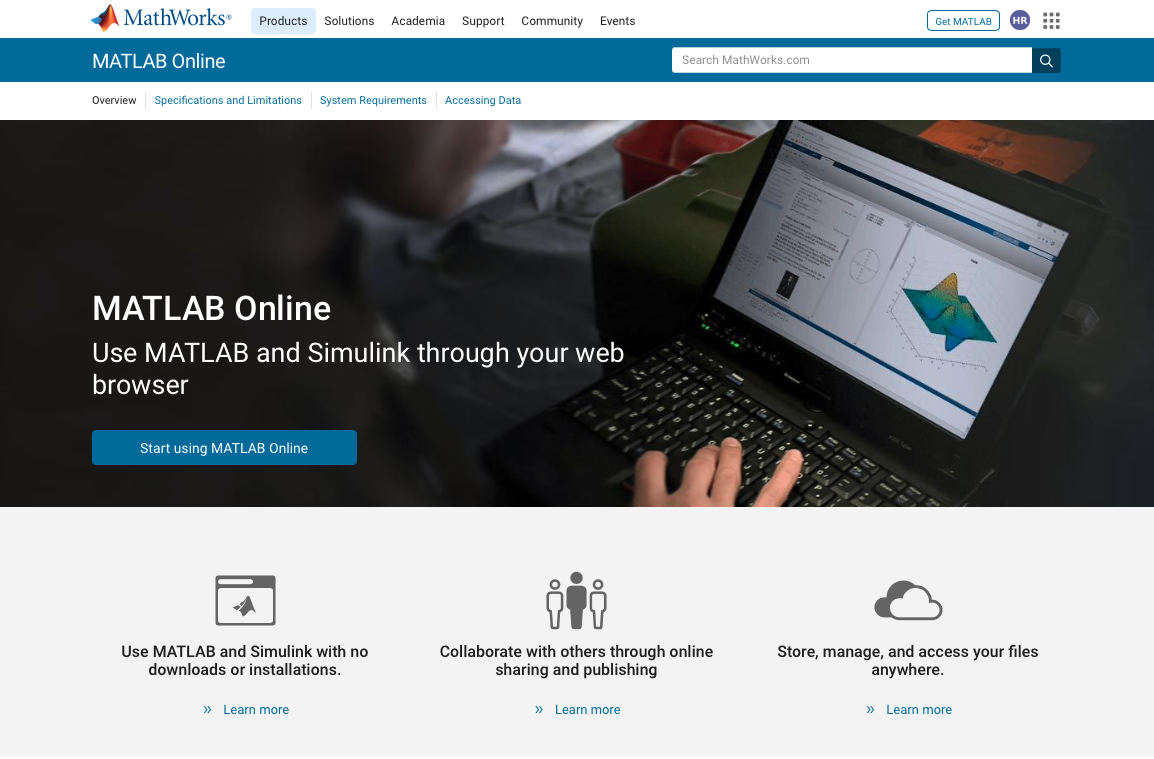
\includegraphics[width=0.9\textwidth]{matlab_online}
\end{center}
\url{https://matlab.mathworks.com}
\end{frame}



\begin{frame}{MATLAB Graphical Interface}
\begin{columns}
\begin{column}[T]{0.35\textwidth}
\begin{itemize}
	\item Command window
	\item Workspace
	\item Current folder
	\item Command history
	\item Editor
	\end{itemize}
\end{column}
\begin{column}[T]{0.75\textwidth}
	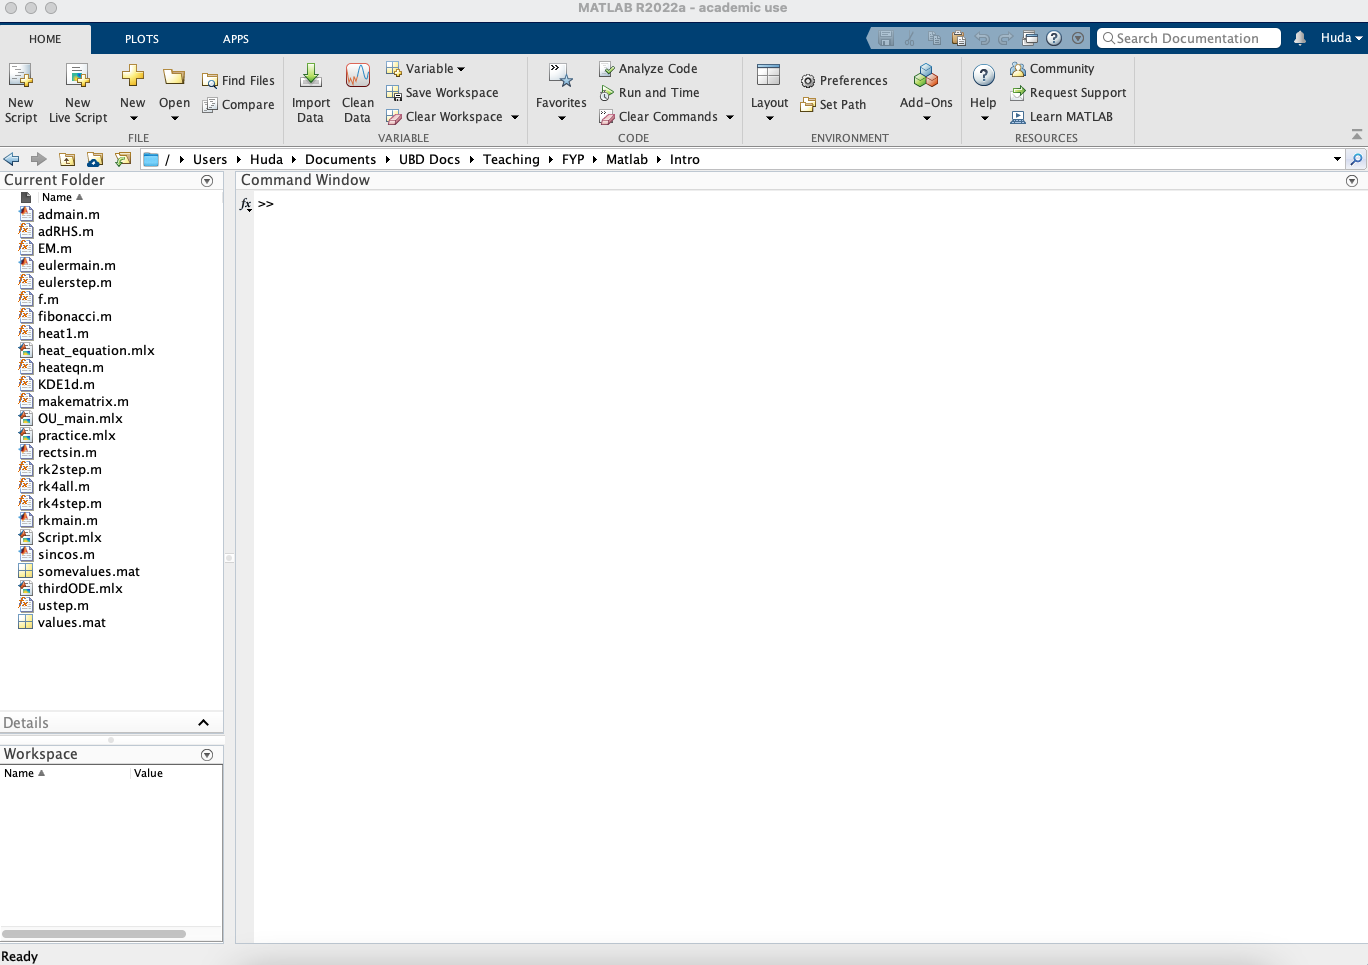
\includegraphics[width=0.9\textwidth]{initial_matlab}
\end{column}
\end{columns}




\end{frame}


%\include{Matlab1}
%\include{Matlab2}
%\include{Matlab3}
%\include{Matlab4}
\end{document}

